\problem{Talking About Numbers}

%\begin{wrapfigure}{r}{0.5\linewidth}
%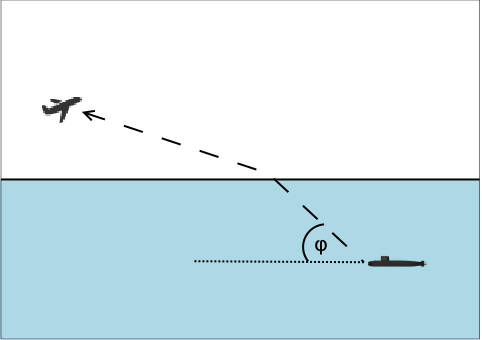
\includegraphics[width=\linewidth]{Refract/refract.png}
%\end{wrapfigure}

The programmers of a TTS (text-to-speech) program have discovered that
their product does a poor job of reading numbers written in
conventional numeric form. Currently, it just announces each digit in
the number, one after the other, which gets confusing to the listener
after a few digits have gone by.

They would prefer to have a more natural reading of numbers, and one
of them has suggested that, if they convert numeric strings into the
appropriate text equivalent, e.g., convert ``1023'' into ``one
thousand and twenty three'', then their speech engine will be able to
handle the reading with no further modification.

Write a program to carry out the transformation of non-negative
integers into conventional English wording:

\begin{itemize}

\item English has unique names for the numbers 0-19: ``zero'',
  ``one'', ``two'', ``three'', ``four'', ``five'', ``six'', ``seven'',
  ``eight'', ``nine'', ``ten'', ``eleven'', ``twelve'', ``thirteen'',
  ``fourteen'', ``fifteen'', ``sixteen'', ``seventeen'', ``eighteen'',
  ``nineteen''.

\item The subsequent multiples of 10 are named ``twenty'', ``thirty'',
  ``forty'', ``fifty'', ``sixty'', ``seventy'', ``eighty'', ``ninety''.

\item The combination of one of those multiples of ten with a digit
  1-9 is always hyphenated: e.g., $31 \Rightarrow$ ``thirty-one'', $77
  \Rightarrow$ ``seventy-seven''.

\item Multiples of 100 are counted 1-9 and set off from any following
  non-zero digits by 'and': e.g., $200 \Rightarrow$ ``two hundred'',
  $412 \Rightarrow$ ``four hundred and twelve'', $777 \Rightarrow$
  ``seven hundred and seventy-seven''.

\item Thousands and millions are counted off using the above rules to
  form numbers 1-999, and are set off from any non-zero remainder 
  by a comma: e.g., $\num{1253101} \Rightarrow$ ``one million, two hundred
  and fifty-three thousand, one hundred and one''.

\item If a number with a non-empty thousands or millions component is
  followed by a remainder of 1-99, then instead of a comma the parts
  are separated by ``and'': e.g., $\num{1000011} \Rightarrow$ ``one
  million and eleven'', $\num{20222043} \Rightarrow$ ``twenty million, two
  hundred and twenty-two thousand and forty-three''.
\end{itemize}

\subsection*{Input}

Input will consist of one or more datasets. Each dataset will consist
of a single line containing a non-negative integer in the range
$0\ldots \num{999999999}$. Although we have used commas within digit
strings for clarity in this problem description, there will be no
commas in the input. There will be no leading zeros on positive input
numbers.

A line with a negative value signals the end of input.

\subsection*{Output}

For each dataset, print a single line containing the spelled-out
equivalent of the number, according to the rules above.

Formatting requirements:
\begin{itemize}
\item The output must be left-justified.
\item All alphabetic characters must be in lower-case.
\item Exactly one blank must separate adjacent words, except when a
  hyphen or comma is called for.
\item When a comma is used, it must be followed by exactly one blank.
\item When a hyphen is used, no blank space appears to either side of
  the hyphen.
\end{itemize}


\subsection*{Example}

Given the input:

\verbfile{TalkingNumbers/test0.in}


the output should be:

\verbfile{TalkingNumbers/test0.expected}



